\documentclass[12pt]{book}
\usepackage[margin=.85in]{geometry} % for MARGIN
\usepackage[many]{tcolorbox}    	% for COLORED BOXES (tikz and xcolor included)


\usepackage{multicol}   
\usepackage{enumerate}
\usepackage[shortlabels]{enumitem}
\usepackage{varwidth}
\usepackage{tasks}
\usepackage[export]{adjustbox}

\usepackage{titleps}
\usepackage{setspace}               % for LINE SPACING
\usepackage[⟨options⟩]{fancyhdr}
\usepackage{enumitem}
\setlist{nosep}
\usepackage{tikz}
\usepackage{pgfplots}
\pgfplotsset{compat=1.5.1}
\usetikzlibrary{datavisualization}
\usetikzlibrary{datavisualization.formats.functions}

\newcommand{\D}{\displaystyle}


\setlength\parindent{0pt}   % killing indentation for all the text
\setstretch{1.3}            % setting line spacing to 1.3
\setlength\columnsep{0.25in} % setting length of column separator
\pagestyle{fancy}           % setting pagestyle to be headings

\usepackage[]{titlesec}

\fancyhead[L]{Math V04 - College Algebra}
\fancyhead[R]{Christina Papazacharioudakis}

\tcbset{
    sharp corners,
    colback = white,
    before skip = 0.2cm,    % add extra space before the box
    after skip = 0.5cm      % add extra space after the box
}                           % setting global options for tcolorbox

    \newtcolorbox{boxR}{
    fontupper = \color{black}, % font color
    boxrule = 1.5pt,
    colframe = black,
    rounded corners,
    arc = 5pt   % corners roundness
}

\definecolor{ballblue}{rgb}{0.13, 0.67, 0.8}

\begin{document}

Name: \underline{\hspace{100mm}}
\vspace{20mm}


\centerline{\Large \textbf{Chapter 2: Equations and Inequalities} } 

{\large
\begin{center}
\begin{varwidth}{\textwidth}
\begin{enumerate}[2.1]
    \item The Regular Coordinate System and Graphs
    \item Linear Equations in One Variable
    \item Models and  Applications (Skipping)
    \item Complex Numbers
    \item Quadratic Equations
    \item Other Types of Equations
    \item Linear Inequalities and Absolute Value Inequalities
\end{enumerate}
\end{varwidth}
\end{center}

}


\newpage
\textbf{{\Large 2.1 The Rectangular Coordinate System and Graphs}}
\vspace{5mm}


{\large \textbf{Plotting Ordered Pairs in the Cartesian Coordinate System }}
\vspace{3mm}

The \textbf{Cartesian coordinate system} is a grid system that has perpendicular axes. The horizontal axis is called the \underline{\hspace{25mm}} and the vertical axis is called the \underline{\hspace{25mm}}. Together, these axes create four sections called quadrants.

\vspace{5mm}

\begin{center}
    
\begin{tikzpicture}[scale=.6, transform shape]
\begin{axis}[
    ymin=-9,
    ymax=9,
    xmin=-9,
    xmax=9,
    axis on top=true,
    axis x line=middle,
    axis y line=middle,
    axis line style={latex-latex},
    xlabel=$$,
    ylabel=$$,
    xticklabels=\empty,
    yticklabels=\empty,
    stick distance=2,
    ytick distance=2,
    axis equal = true, 
    every axis x label/.style={at={(ticklabel* cs:1.0)}, anchor=west,},
    every axis y label/.style={at={(ticklabel* cs:1.0)}, anchor=south,}
]
    \pgfplotsset{ticks=none}
\end{axis}
\end{tikzpicture}
\end{center}
\vspace{5mm}

The center of the plane is where the two axis cross. This is known as the {\underline{ \hspace{20mm}}}. 


A point in the plane is defined as an ordered pair $(\hspace{5mm}, {\hspace{5mm} })$ which tells us how far we have moved from the origin in the $x$ direction (horizontally) and the $y$ direction (vertically). The origin has the point  $(\hspace{5mm}, {\hspace{5mm} })$.

\vspace{5mm}

\underline{\textbf{Example 1 - Plotting Points in a Rectangular Coordinate System}}

Plot the points $(-2,4), (3,3), (0,-3), \text{ and } (-3,0) $.

\begin{center}
    
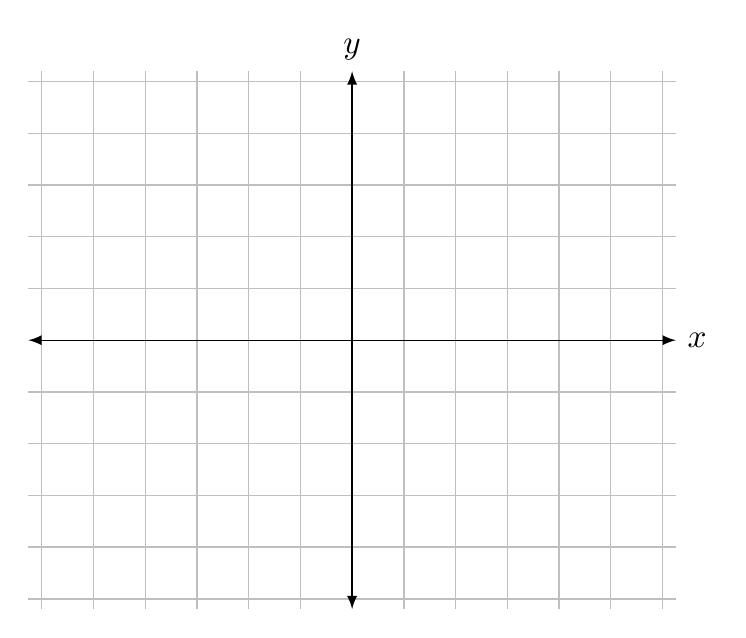
\begin{tikzpicture}[scale=1.2, transform shape]
\begin{axis}[
    ymin=-5.2,
    ymax=5.2,
    xmin=-5.2,
    xmax=5.2,
    axis on top=true,
    axis x line=middle,
    axis y line=middle,
    axis line style={latex-latex},
    xlabel=$x$,
    ylabel=$y$,
    xticklabels=\empty,
    yticklabels=\empty,
    xtick distance=1,
    ytick distance=1,
    xmajorgrids=true,
    ymajorgrids=true,
    axis equal = true, 
    every axis x label/.style={at={(ticklabel* cs:1.0)}, anchor=west,},
    every axis y label/.style={at={(ticklabel* cs:1.0)}, anchor=south,}
]
    \pgfplotsset{ticks=none}
\end{axis}
\end{tikzpicture}
\end{center}


\newpage
{\large \textbf{Graphing Equations by Plotting Points}}
\vspace{3mm}

\begin{boxR}
    \textbf{How To}
    \vspace{1mm}
    \hline
      \vspace{2mm}
   \textbf{ Given an equation, graph by plotting points.}
    \begin{enumerate}
        \item Make a table with one column labeled $x$, a second column labeled with the equation, and a third column listing the resulting ordered pairs.
        \item Enter $x$-values down the first column using positive and negative values. Selecting the x-values in numerical order will make the graphing simpler.
        \item Select x-values that will yield y-values with little effort, preferably ones that can be calculated mentally.
        \item Plot the ordered pairs.
        \item Connect the points if they form a line.

    \end{enumerate}
\end{boxR}

\underline{\textbf{Example 2 - Graphing Equations by Plotting Points}}

Graph the equation $y=-x+2$ by plotting points.

\vspace{70mm}
\par 
\begin{raggedleft}
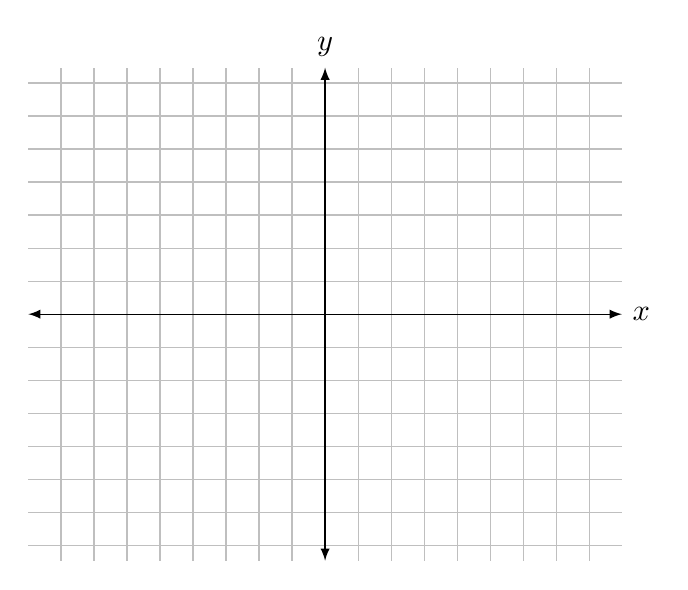
\begin{tikzpicture}[scale=1.1, transform shape]
\begin{axis}[
    ymin=-11.2,
    ymax=11.2,
    xmin=-11.2,
    xmax=11.2,
    axis on top=true,
    axis x line=middle,
    axis y line=middle,
    axis line style={latex-latex},
    xlabel=$x$,
    ylabel=$y$,
    xticklabels=\empty,
    yticklabels=\empty,
    xtick distance=1.5,
    ytick distance=1.5,
    xmajorgrids=true,
    ymajorgrids=true,
    axis equal = true, 
    every axis x label/.style={at={(ticklabel* cs:1.0)}, anchor=west,},
    every axis y label/.style={at={(ticklabel* cs:1.0)}, anchor=south,}
]
    \pgfplotsset{ticks=none}
\end{axis}
\end{tikzpicture}
\par
\end{raggedleft}

\newpage


{\large \textbf{Finding x-intercepts and y-intercepts}}

\begin{boxR}
    \textbf{How To}
    \vspace{1mm}
    \hline
      \vspace{2mm}
   \textbf{ Given an equation, find the intercepts.}
    \begin{itemize}
        \item Find the $x$-intercept by setting $y=0$ and solving for $x$.
        \item Find the $y$-intercept by setting $x=0$ and solving for $y$.
    \end{itemize}
\end{boxR}
\vspace{3mm}

\underline{\textbf{Example 4 - Finding the Intercepts of the Given Equation}}
Find the intercepts of the equation $y=-3x-4$. Then sketch the graph using only the intercepts. 

\vspace{100mm}
\par 
\begin{raggedleft}
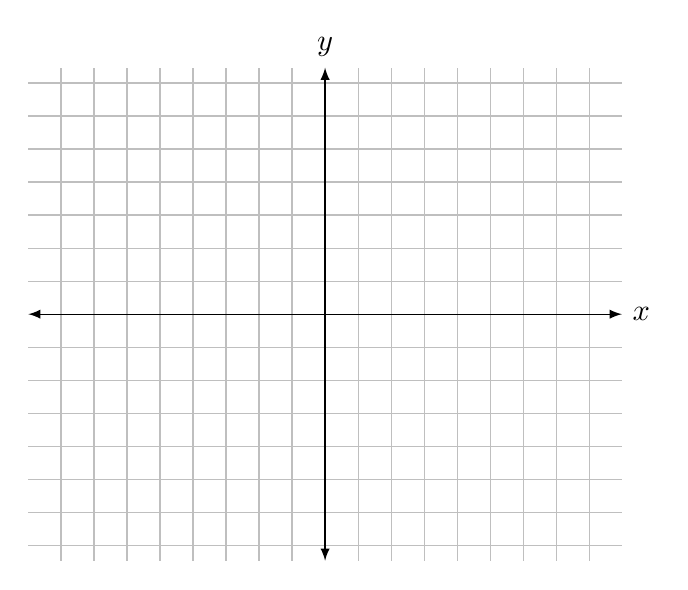
\begin{tikzpicture}[scale=1.1, transform shape]
\begin{axis}[
    ymin=-11.2,
    ymax=11.2,
    xmin=-11.2,
    xmax=11.2,
    axis on top=true,
    axis x line=middle,
    axis y line=middle,
    axis line style={latex-latex},
    xlabel=$x$,
    ylabel=$y$,
    xticklabels=\empty,
    yticklabels=\empty,
    xtick distance=1.5,
    ytick distance=1.5,
    xmajorgrids=true,
    ymajorgrids=true,
    axis equal = true, 
    every axis x label/.style={at={(ticklabel* cs:1.0)}, anchor=west,},
    every axis y label/.style={at={(ticklabel* cs:1.0)}, anchor=south,}
]
    \pgfplotsset{ticks=none}
\end{axis}
\end{tikzpicture}
\par
\end{raggedleft}


\newpage

{\large \textbf{Using the Distance Formula}}

Derived from the \underline{\hspace{50mm}}, the distance formula is used to find the distance between two points in the plane. Let's take a closer look! 

\vspace{150mm}




\begin{boxR}
\textbf{The Distance Formula}
 \vspace{1mm}
    \hline
      \vspace{2mm}
Given the endpoints $(x_1,y_1)$ and $(x_2, y_2)$m the distance between two points is given by 

    $$ d= \sqrt{(x_2-x_1)^2 + (y_2-y_1)^2}$$
\end{boxR}
\newpage

\underline{\textbf{Example 5 - Finding the Distance Between Two Points}}

Find the distance between the points $(-3, -1)$ and $(2,3)$.


\vspace{40mm}
{\large \textbf{Using the Midpoint Formula}}
When the endpoints of a line segment are known, we can find the point that is midway between them. 
\vspace{2mm}
\begin{boxR}
\textbf{Midpoint Formula}
 \vspace{1mm}
    \hline
      \vspace{2mm}
Given the endpoints of a line segment $(x_1,y_1)$ and $(x_2, y_2)$, the coordinate of the midpoint $M$ is given by

    $$ M= \left(\frac{x_1 + x_2}{2}, \frac{y_1+y_2}{2}\right)$$
\end{boxR}

\newpage


\underline{\textbf{Example 7 - Finding the Midpoint of a Line Segment}}

Find the midpoint of the line segment with the endpoints $(7, -2)$ and $(9,5)$.


\vspace{70mm}
\underline{\textbf{Example 8 - Finding the Center of a Circle}}

The diameter of a circle has endpoints $(-1,-4)$ and $(5,-4)$. Find the center of the circle. 
\newpage
\textbf{{\Large 2.2 Linear Equations in One Variable}}
\vspace{5mm}


{\large \textbf{Solving Linear Equations in One Variable}}
\vspace{3mm}

A \textbf{linear equation} in one variable can be written in the form \underline{\hspace{25mm}} where $a$ and $b$ are real numbers, $a \neq 0$. 

\vspace{3mm}

\underline{\textbf{Example 1 - Solving an Equation in One Variable}}

\vspace{1mm}
Solve the equation: $\D 2x+7 = 9$.

\vspace{60mm}
\underline{\textbf{Example 2 - Solving an Equation Algebraically When the Variable Appears on Both Sides}}

\vspace{1mm}
Solve the following equation: $\D 4(x-3) + 12 = 15-5(x+6)$.


\newpage

\begin{boxR}
    \textbf{How To}
    \vspace{1mm}
    \hline
      \vspace{2mm}
   \textbf{Given a linear equation in one variable, use algebra to solve it.} Our goal is to have the last line read ``$x$\hspace{1mm}=\hspace{1mm}\underline{\hspace{10mm}}"

Depending on what we are given, we might need to use the following steps:
    \begin{enumerate}
     \item We may add, subtract, multiply, or divide an equation by a number or an expression to both sides of the equal sign. Note that we cannot divide by zero.
     \item Apply the distributive property as needed: $a(b+c)=ab+ac$.
     \item Isolate the variable on one side of the equation.
       \end{enumerate}
\end{boxR}
\vspace{3mm}
{\large \textbf{Solving a Rational Equation}}

We now look at rational equations, which are secretly linear equations after some algebra manipulation. 
\vspace{5mm}
A \textbf{rational equation} is an equation that contains at least one rational expression. 

Examples of rational expressions:

$$\frac{x+1}{x^2-4}, \frac{1}{x-3}, \text{ or } \frac{4}{x^2+x-2}$$
\vspace{3mm}

What makes them a rational expression? 

\vspace{15mm}
\begin{boxR}
    \textbf{How To}
    \vspace{1mm}
    \hline
      \vspace{2mm}
   \textbf{Given a rational equation, solve it.} 

    \begin{enumerate}
     \item Factor all denominators in the equation.
     \item Find the LCD.
     \item Multiply the entire equation by the LCD. If the LCD is correct, there will be no denominators left.
     \item Solve the remaining equation.
     \item Make sure to check solutions back in the original equations to avoid a solution producing zero in a denominator.
       \end{enumerate}
\end{boxR}
\newpage
\underline{\textbf{Example 3 - Solving a Rational Equation}}

\vspace{1mm}
Solve the rational equation: $\D \frac{7}{2x}-\frac{5}{3x}=\frac{22}{3}$.
\newpage

\underline{\textbf{Example 4 - Solving a Rational Equation without Factoring}}

\vspace{1mm}
Solve the rational equation: $\D \frac{2}{x}-\frac{3}{2}=\frac{7}{2x}$

\vspace{80mm}
\underline{\textbf{Example 5 - Solving a Rational Equation by Factoring the Denominator}}

\vspace{1mm}
Solve the rational equation: $\D \frac{1}{x}=\frac{1}{10}-\frac{3}{4x}$

\newpage
\underline{\textbf{Example 6 - Solving Rational Equations with a Binomial in the Denominator}}

\vspace{1mm}
Solve the following rational equations and state the excluded values:
\vspace{1mm}
\begin{enumerate}[(a)]
    \item $\D \frac{3}{x-6} = \frac{5}{x}$
    \vspace{100mm}
    \item $\D \frac{x}{x-3} = \frac{5}{x-3} - \frac{1}{2}$
    
\end{enumerate}
\newpage
\underline{\textbf{Example 7 - }} 

\underline{\textbf{Solving a Rational Equation with Factored Denominators and Stating Excluded Values}}
Solve the rational equation after factoring the denominators: 
$$ \frac{2}{x+1} - \frac{1}{x-1} = \frac{2x}{x^2-1} $$

\newpage

{\large \textbf{Finding a Linear Equation}}

The most familiar form of a line equation is the \textbf{slope-intercept form}, written as $y=mx+b$, where $m =$ slope and $b = $ y-intercept. 

\vspace{90mm}
Lets begin with finding the slope! 

The $slope$ of a line refers to the ratio of vertical change in $y$ over the horizontal change in $x$. 



\newpage
{\large \textbf{The Slope of a Line}}

\begin{boxR}
    \textbf{The Slope of a Line}
    \vspace{1mm}
    \hline
      \vspace{2mm}

   The slope of a line, $m$, represents the change in $y$ over the change in $x$. Given two points $(x_1,y_1)$ and $(x_2,y_2)$, the slope $m$ is $$ m = \frac{y_2-y_1}{x_2-x_1}$$
\end{boxR}

\vspace{2mm}
\underline{\textbf{Example 8 - Finding the Slope of a Line Given Two Points}}

Find the slope of a line that passes through the points $(2,-1)$ and $(-5,3)$.

\vspace{60mm}
\underline{\textbf{Example 9 - Identifying the Slope and y-Intercept Given the Equation of a Line}}

\vspace{1mm}
Identify the slope and $y$-intercept in $\D y= \frac{-3}{4}x -4$

\newpage 


{\large \textbf{The Point-Slope Formula}}

If we know the slope of a line and a point that is passes through (not the y-intercept), we can still find the equation of a line.

\vspace{3mm}
\begin{boxR}
    \textbf{The Point-Slope Formula}
    \vspace{1mm}
    \hline
      \vspace{2mm}
      Given one point $(x_1,y_1)$ and a slope, the point-slope formula of a line is

      $$ y-y_1 = m(x-x_1)$$
\end{boxR}

\vspace{2mm}

\underline{\textbf{Example 10 - Finding the Equation of a Line Given the Slope and One Point}}

Write the equation of a line with slope $m=-3$ passing through the point $(4,8)$. Write your final equation in slope-intercept form.

\vspace{60mm}

\underline{\textbf{Example 11 - Find the Equation of a Line Passing Through Two Given Points}}

Find the equation of a line passing through the points $(3,4)$ and $(0,-3)$. Write your final equation in slope-intercept form.

\newpage

{\large \textbf{Standard Form of a Line}}

Another way we can represent the equation of a line is in standard form. 

\begin{boxR}
    \textbf{Standard Form of a Line}
    \vspace{1mm}
    \hline
      \vspace{2mm}
      The standard form of a line is given as
      $$ Ax + By = C $$
      where $A, B$, and $C$ are integers. 
\end{boxR}

\underline{\textbf{Example 12 - Find the Equation of a Line and Writing It in Standard Form}}

Find the equation of a line with $m=-6$ passing through the point $\left(\frac{1}{4},-2\right)$. Write the equation in standard form.

\vspace{60mm}

{\large \textbf{Vertical and Horizontal Lines}}

\begin{boxR}
    The equation of a vertical line is given as $x=c$. The slope of a vertical line is not defined.

    The equation of a vertical line is given as $y=c$. The slope of a horizontal line is zero.
\end{boxR}

\newpage


\underline{\textbf{Example 13 - Find the Equation of a Line Passing Through the Given Points}}

Find the equation of a line passing through the points $(1,-3)$ and $(1,4)$.

\vspace{60mm}

{\large \textbf{Determining Whether Graphs of Lines are Parallel or Perpendicular}}

Parallel lines have the \underline{\hspace{20mm}} slope but \underline{\hspace{20mm}} y-intercepts.

Perpendicular lines intersect to form a $90^\circ$ angle. The slope of one line is the negative reciprocal of the other. 


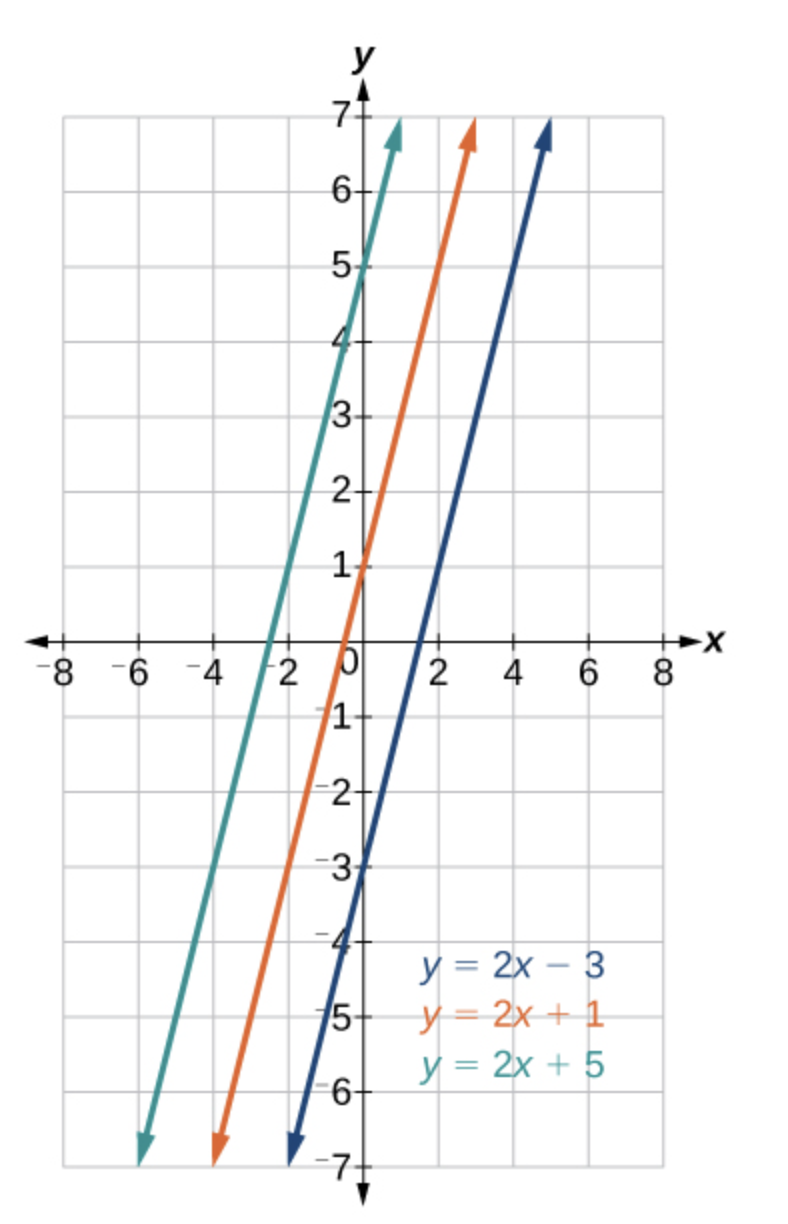
\includegraphics[height=100mm, width=70mm]{2.2 FIg 4.png}
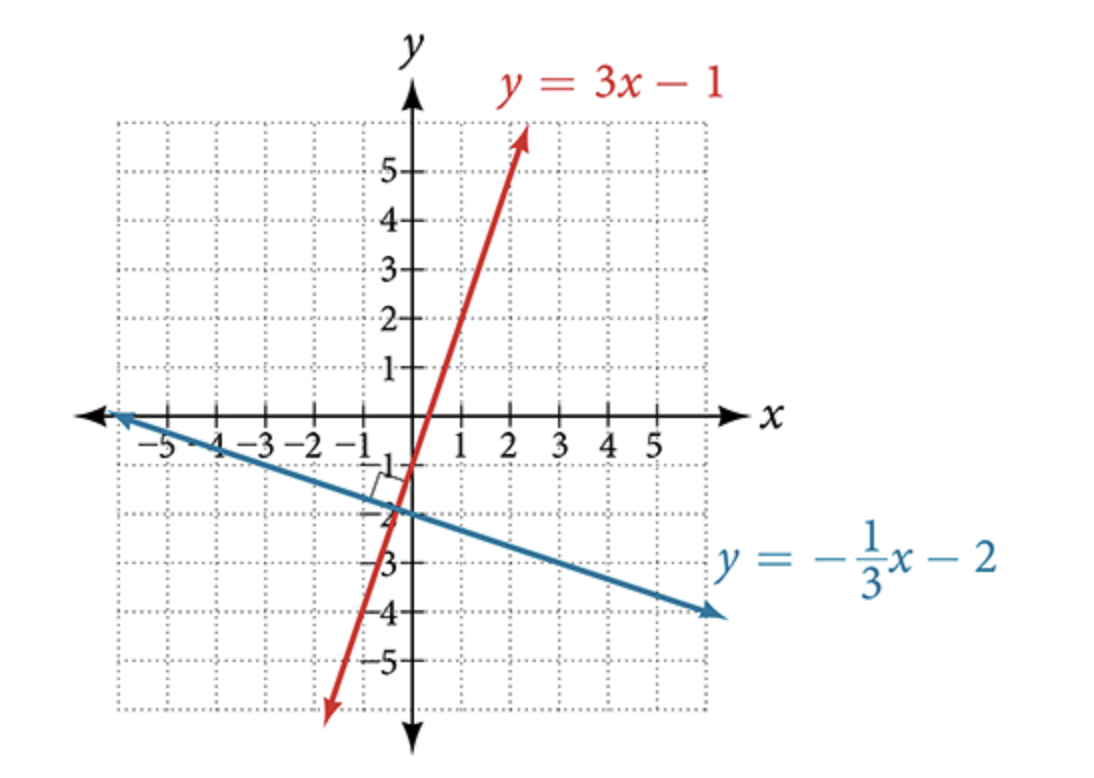
\includegraphics[height=80mm, width=100mm]{2.2 Fig 5.png}

\newpage
\underline{\textbf{Example 14 - Graph Two Lines to Determine Parallel, Perpendicular, or Neither}}

Graph the equations of the given lines and determine if they are parallel, perpendicular, or neither. 
$$ 3y=-4x+3 \text{ and } 3x-4y=8$$

\vspace{3mm}
\begin{center}

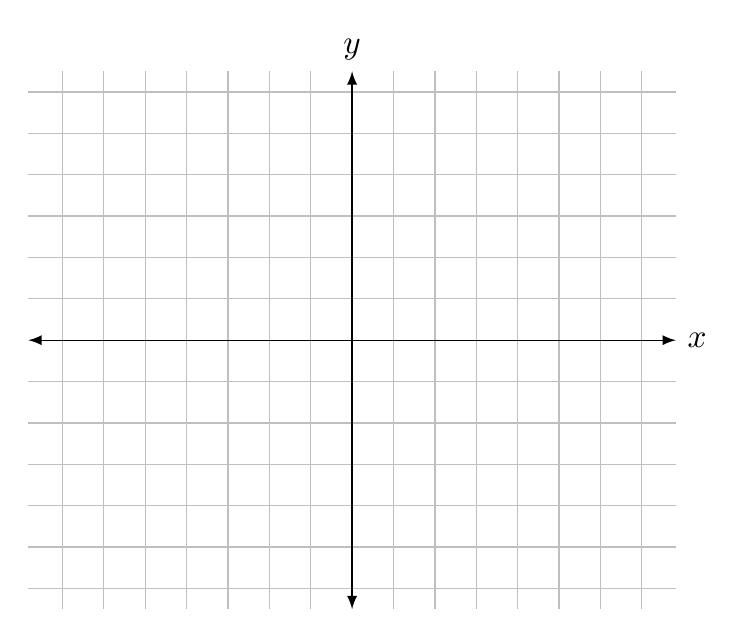
\begin{tikzpicture}[scale=1.2, transform shape]
\begin{axis}[
    ymin=-6.5,
    ymax=6.5,
    xmin=-6.5,
    xmax=6.5,
    axis on top=true,
    axis x line=middle,
    axis y line=middle,
    axis line style={latex-latex},
    xlabel=$x$,
    ylabel=$y$,
    xticklabels=\empty,
    yticklabels=\empty,
    xtick distance=1,
    ytick distance=1,
    xmajorgrids=true,
    ymajorgrids=true,
    axis equal = true, 
    every axis x label/.style={at={(ticklabel* cs:1.0)}, anchor=west,},
    every axis y label/.style={at={(ticklabel* cs:1.0)}, anchor=south,}
]
    \pgfplotsset{ticks=none}
\end{axis}
\end{tikzpicture}
\end{center}

\newpage

\begin{boxR}
    \textbf{How To}
    \vspace{1mm}
    \hline
      \vspace{2mm}
      \textbf{Given an equation for a line, write an equation of a line parallel or perpendicular to it.}
     \begin{enumerate}
         \item  Find the slope of the given line. The easiest way to do this is to write the equation in slope-intercept form.
         \item Use the slope and the given point with the point-slope formula.
         \item Simplify the line to slope-intercept form and compare the equation to the given line.
         \end{enumerate}
\end{boxR}
\vspace{2mm}

\underline{\textbf{Example 15 \& 16 - Finding a Parallel and Perpendicular Line}}

Find the equation of a line passing through the point  $(3,5)$ that is 
\begin{enumerate}[(a)]
    \item parallel to $5x+3y=1$.
    \item perpendicular $5x+3y=1$.
\end{enumerate}



\vspace{145mm}
Notes for section 2.4-2.7 to come... stay tuned!

\end{document}


